\documentclass{article}
\usepackage[utf8]{inputenc}
\usepackage{amsmath,empheq}
\usepackage{graphicx}
\usepackage{gensymb}
\usepackage{mathtools}
\usepackage{subfig}
\usepackage[margin=2.5cm]{geometry}
\usepackage{graphicx}
\def\plus{\texttt{+}}
\def\minus{\texttt{-}}

\title{Control Theory}
\author{Toon Dewindt \\
Mathieu Delforge }
\date{November 2019}

\begin{document}

\maketitle
\clearpage
\section{Abstract}
\clearpage
\tableofcontents
\listoffigures
\clearpage
\section{Introduction}
This document will tackle the topic of analysing and controlling an electrical cart by use of theoretical models and practical experiments. This specific cart is driven by two electrical DC motors that are controlled by an arduino board which is mounted on the cart itself. On this cart is also a pendulum of which the angle can be measured by a sensor. A second sensor is mounted on the front of the cart and measures the distance. The angle of this sensor can be changed.\\
\\
The goals of this task is the identification of the engines, the transferfunction, ...



\section{Identification of the engine}
\subsection{Theoretical model of the DC engine}
The first step of the entire proces is determining the ideal theoretical behavior of the motors. This behavior is based on the idealised internal construction of the DC-motor and can be viewed in figure \ref{fig:DC-motor_elektrisch}. To be able to write down the transfer function of the system, the equations that govern this electrical system need to be written down. From the manipulation of these equations it is possible to get the transfer function. The obtained functions are based on the very basic equations that govern an electical system: the laws of Kirchoff. The following equations are obtained.
\begin{figure}
    \centering
    \includegraphics[scale=0.8]{{"pics assignment 1/DCmotor_el"}}
    \caption{Electrical scheme of a DC motor}
    \label{fig:DCmotor}
\end{figure}
\begin{equation}
\label{eq:kirchoff}
\begin{split}
    V_{a} - R_{a}i - L_{a}\frac{di}{dt} - V_{c} = 0 \\
    V_{c} = K_{1} \omega \\
    J\frac{d\omega}{dt} + f\omega = K_{2}i
\end{split}
\end{equation}
With
\begin{itemize}
    \item $K_{1}$ = back emf constant 
    \item $K_{2}$ = torque constant
    \item f = friction coëfficient of the engine [$\frac{Nm}{\frac{rad}{s}}$]
    \item J = Inertia of the rotor
\end{itemize}
By converting these functions to the s-domain and the use of a bit of mathematical wizardry, the theoretical transfer function obtained (cfr. eq \ref{eq:theoretische transferfunctie}). This transfer function uses the voltage source given by the arduino board ($V_{a}$). The output is the rotational speed of the engine ($\omega$). The transfer function of these in- and outputs is then
\begin{equation}
\label{eq:theoretische transferfunctie}
    \frac{\omega}{V} = \frac{K_{2}}{L_{a}Js^2 + (L_{a}f + R_{a}J)s + R_{a}f+K_{1}K_{2}}
\end{equation}
From this transfer function the poles and zeros can be calculated. The poles of the system are the s values for which the transfer function goes to infinity, so the values for which the denominator becomes zero. The zeros are the values for which the transfer function becomes zero, so the values for which the numerator is zero. It is easy to see that this specific function has no zeros. The poles can be easily calculated by solving the second degree equation. The obtained values are then

\begin{itemize}
\label{it:polen van het systeem}
    \item $s_{1}$ = $\frac{-(L_{a}f+R_{a}J) + \sqrt((L_{a}f+R_{a}J)^2-4L_{a}JK_{1}K_{2})}{L_{a}J}$
    \item $s_{2}$ = $\frac{-(L_{a}f+R_{a}J) - \sqrt((L_{a}f+R_{a}J)^2-4L_{a}JK_{1}K_{2})}{L_{a}J}$
\end{itemize}

\\
The input of the system is the voltage that is connected to the engine and is determined by the arduino program/board. The unit of the input is volt. The output is the angular velocity of the engine and its unit is rad/s. The states are angular velocity [rad/s] and electrical current [A].\\
\\
To make life easier certain effects of the engine can be neglected: the value of the coil ($L_{a}$) because it is small compared to the other values in the system. After this change the following transfer function is obtained.\cite{handboek}
\begin{equation}
\label{eq:transferfunctie eenvoudig}
    \frac{\omega}{V} = \frac{K_{2}}{R_{a}Js+R_{a}f+K_{1}K_{2}}
\end{equation}
With this simplified equation it is now possible to move to the next step: turning this continuous equation to a discrete one. The used method is the backward Euler method.  This is done by changing out the s for $\tfrac{z-1}{T_{s}z}$, with now z being the discrete domain variable and $T_{s}$ the time between two samples. After simplification the new time-discrete transfer function is obtained.
\begin{equation}
\label{eq:transferfunctie discreet}
    \frac{\omega}{V} = \frac{K_{2}T_{s}z}{(R_{a}J+R_{a}fT_{s}+K_{1}K_{2}T_{s})z-R_{a}J}
\end{equation}
\subsection{Transfer function of the engine itself}
In order to be able to get the real transfer function of the engine itself an excitation is needed. The excitation signal should be developed in such a way that it is long enough for the transient response to die out so that only the steady state response is left. A last requirement is that as many frequencies as possible have to be used.\\
\\
Taking all these requirements into account the chosen excitation signal is a block puls that starts at zero, goes up to 5 volts and back to zero. The first requirement is achieved by running the high voltage for four seconds. The second requirement is obtained by using the block puls - a block puls transformed to the frequency domain is a sinc pulse which has all the useful frequencies-. The excitition signal is shown in figure \ref{fig:excitationsignal}. On this figure the respons of the motor is also plotted. Small variations can be seen when the voltage is at it's maximum.\\
\\
During the process of applying a signal and measuring the output random noise is introduced. This noise can be minimised by repeating the signal and then overlaying these outputs. Due to this the random noise is filtered out and a clearer output signal is obtained\\
\\
\begin{figure}
    \centering
    \includegraphics[scale=0.7]{{"pics assignment 1/excitation_signal"}}
    \caption{Block puls excitation signal and the angular velocity respons}
    \label{fig:excitationsignal}
\end{figure}
In order to be able to compare the empirical system with the theoretical system they have to be of the same order. For this reason the following transfer function is chosen.
\begin{equation}
    H(z) = \frac{az}{z+b}
\end{equation}
In order to be able to write down a recursion expression, the transfer function (equation (5)) needs to be transformed to the time discrete domain. The following expression is obtained.
\begin{equation}
    y[k] = - by[k-1] + au[k]
\end{equation}
In order to make use of all the obtained data and minimise noise, the average of the responses of the five block pulses is calculated. This new data is then used to make matrix A and B. 
\begin{equation}
    B = A[b\:a]^T
\end{equation}
with
\begin{itemize}

    \item A = 
        $\begin{bmatrix}
            - y[0] & u[1] \\
            - y[1] & u[2] \\
            . & .\\
            . & .\\
            - y[k-1] & u[k]
        \end{bmatrix}$
    \item B = 
        $\begin{bmatrix}
            y[1] \\
            y[2] \\
            . \\
            . \\
            y[k]
        \end{bmatrix}$

\end{itemize}
The error criterion that minimises this expression is??\\
\\
The obtained transfer functions are then the following\\
\begin{equation}
    \frac{\omega_{A}}{V} = \frac{0.4303z}{z-0.7988}  
\end{equation}
\begin{equation}
    \frac{\omega_{B}}{V} = \frac{0.4206z}{z-0.7989}
\end{equation}
\\
Due to the low sampling frequency a lot of high frequency noise is introduced. This and other noise can be filtered out with well a filter. The chosen one in this assignment is the buttersworth filter. Another name for this filter is "maximally flat magnitude filter" which shows the first useful property of this filter: it has a uniform sensitivity for the wanted frequencies. The second useful property of this filter is that it rejects higher frequencies that are unwanted.\\
\\
The characteristics of this filter are the following. Buttersworth filter of the sixth order with a cut-off frequency of six Hz.\\
\\
After filtering the poles and zeros of the estimated transfer function have changed. The new transferfunctions are shown here.
\begin{equation}
    \frac{\omega_{A_{filtered}}}{V} = \frac{0.4945z}{z-0.7691}  
\end{equation}
\begin{equation}
    \frac{\omega_{B_{filtered}}}{V} = \frac{0.4206z}{z-0.7672}
\end{equation}
The new poles and zeros are then
\begin{itemize}
\centering
    \item $zero_{A}$ = 0
    \item $pole_{A}$ = 0.7691
    \item $zero_{B}$ = 0
    \item $pole_{B}$ = 0.7672
\end{itemize}
Figure \ref{fig:poles and zeros} shows the poles and zeros of the system before and after the filtering of the data.
\begin{figure}
    \centering
    \includegraphics[scale=0.7]{{"pics assignment 1/Poolmap_filtervsUnfilter"}}
    \caption{The poles and zeros of the transfer functions before (blue) and after (red) filtering of motor A}
    \label{fig:poles and zeros}
\end{figure}
\\
After these calculations there are three responses: the response of the motor itself (the empirical data), the non filtered data and the last being the filtered data. All three of these responses of motor A are shown in figure \ref{fig:bodetfmotorA} and the same ones of motor B are shown in figure \ref{fig:bodetfmotorB}. \\

\begin{figure}
    \centering
    \includegraphics[width=\linewidth, height=5cm]{{"pics assignment 1/transfer_MotorA"}}
    \caption{Bode plot of the different transferfunctions of motor A}
    \label{fig:bodetfmotorA}
\end{figure}
\begin{figure}
    \centering
    \includegraphics[width=\linewidth, height=5cm]{{"pics assignment 1/transfer_MotorB"}}
    \caption{Bode plot of the different transferfunctions of motor B}
    \label{fig:bodetfmotorB}
\end{figure}
\\
To validate the model a step input is used on both the actual engine and on the transfer function (based on the filtered signals) and its response is then measured. To be able to compare the output of both transfer functions, the input has to be the same. The step function in matlab can be simulated by the command lsim(). Both outputs and the difference for motor A are given in figure \ref{fig:stepresponsA}, the same is given for motor B in figure \ref{fig:stepresponsB}. In the beginning there is a huge transient difference. This difference can be attributed to the inertia of the wheel and also that it takes two time steps before voltage is given to the wheels. The differences in the steady state are very small so the estimated and simplified transfer function can be assumed to be close enough to the actual system.\\

\begin{figure}
    \centering
    \begin{minipage}[b]{0.4\linewidth}                                          \includegraphics[scale=0.4]{{"pics assignment 1/step_MotorB"}}
        \caption{Simulated and meaured respons of motor A and the difference}
        \label{fig:stepresponsA}
    \end{minipage}
    \begin{minipage}[b]{0.4\linewidth}
        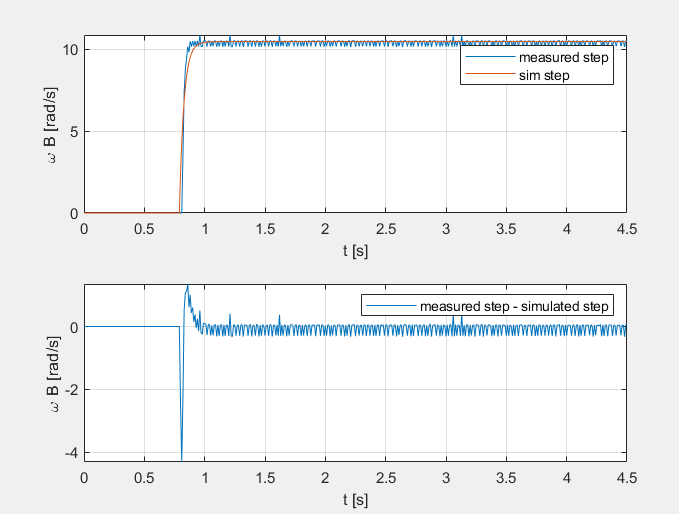
\includegraphics[scale=0.4]{{"pics assignment 1/step_MotorB.PNG}}
        \caption{Simulated and meaured respons of motor B and the difference}
        \label{fig:stepresponsB}
    \end{minipage}
\end{figure}

The superposition principle states that the output of two or more inputs has to be the sum of the responses of these inputs individually. Any function that fulfils these properties is a linear function. The formula form of this principle is the following.
\begin{equation}
    F(ax_{1}+bx_{2}) = aF(x_{1}) + b F(x_{2})
\end{equation}
In this case the different inputs (x) are the voltages applied to the motor and the outputs (F) are the speed of the wheels. 
\\
\\
To see if the transfer function fulfils this principle first an impulse of 1 volt is applied to the engine and it's response is measured, the response being the rotational velocity. Then a second voltage is applied: a five volt signal. After multiplying the output of the one volt signal by five and comparing this with the output of the six volt signal a clear difference is seen. Due to this it is clear to see that the system is non linear. This is also show in figure \ref{fig:nonlin}. The reason for this non linearity are losses in the system. Since the cart is lifted of the ground during the experiment the non-linearity is not due to friction. However there are internal losses such as eddy currents and hysteresis losses that arise due to the commutation of the magnetic field in the armature. \cite{non-linearity in DC-motor}

\begin{figure}
    \centering
    \includegraphics[scale=0.5]{{"pics assignment 1/proof_nonlinear"}}
    \caption{Proof of the non linearity of the system}
    \label{fig:nonlin}
\end{figure}



\subsection{Identification of the cart}
All the previously obtained transfer functions were determined when the wheels were freely spinning in the air. The cart however has to drive on the ground. The obtained model has to be re-evaluated with now the cart on the ground. The validation is done by the same method as before: comparing the output of a step function applied on the cart on the ground and the output of the simulated response of the derived transfer function excited by the same step input. The result is show in figure \ref{fig:groundvsair}.

\begin{figure}[h]
    \centering
    \begin{minipage}[b]{0.4\linewidth}                                          \includegraphics[scale=0.4]{{"pics assignment 1/step_wagen_grond_MotorA"}}
        \caption{measured and simulated response of motor A on the ground}
        \label{fig:stepresponsA}
    \end{minipage}
    \begin{minipage}[b]{0.4\linewidth}
        \includegraphics[scale=0.4]{{"pics assignment 1/step_wagen_grond_MotorB"}}
        \caption{measured and simulated response of motor B on the ground}
        \label{fig:stepresponsB}
    \end{minipage}
\end{figure}

The response of the cart on the ground is different to the simulated response. The reason for this is that now the tyres make contact to the ground and friction is introduced. A second reason is that now the inertia and weight of the cart influence the wheels. For this reason the response of the cart on the ground rises slower than the simulated response of the wheels in the air.\\
\\
The model now has to be re-evaluated. New data is obtained by placing the cart on the ground and applying the same block pulse that was used to identify the respons of the engine when the wheels were lifted of the ground (cfr. fig \ref{fig:excitationsignal}).\\
\\
After using this new data in the matlab code and after filtering, new transfer functions are obtained.
\begin{equation}
    \frac{\omega_A}{V} = \frac{0.05855}{z - 0.9704}
\end{equation}
\begin{equation}
    \frac{\omega_B}{V} = \frac{0.05867}{z - 0.9702}
\end{equation}
The poles and zeros of this function are
\begin{itemize}
\centering
    \item $pole_{A}$ = 0.9704
    \item $zero_{A}$ = 0
    \item $pole_{B}$ = 0.9702
    \item $zero_{B}$ = 0
\end{itemize}
A good engineer always tries to reason what will happen when inputs are changed and then sees if the output of the program matches the expectations. When placing the cart on the ground it is logical to assume that the response will be slower due to the inertia and friction. When looking at the new respons this change is clearly visible.

\clearpage
\section{Controller}
\subsection{choice and design}
The wanted specification for the system is a zero steady state error without changing the filtering of high frequency noise. A stable system is also wanted, for this all the poles -of the continuous transfer function- have to be in the left half plane (LHP). A third requirement is tracking: the output must follow the input as closely as possible. The fourth and last condition is that the error should be small when the reference is at a constant setpoint.\\
\\
These requirements can be achieved by either a PI- or a PID controller. The choice goes to the PI controller for two reasons. The first reason is why the PID is discarded as an option: a PID controller will amplify higher frequencies and this would amplify the noise to very high levels. The second reason is that the PI controller will fulfil all the specifications, so using a PID controller would make the work more complicated and expensive.\\
\\
The requirement of zero steady state error can be fulfilled by making the DC-gain infinite. A drawback of the PI controller is the phase lag that occurs when implementing this type of controller. This phase lag occurs for all frequencies higher than the break frequency ($\frac{1}{T_{i}}$). But by playing and testing different break frequencies the wanted response can be obtained.\\
\\
Designing the PI controller is a process with many steps. The first step is determining the crossover frequency, this frequency is chosen where the uncompensated open loop system has a phase equal to -180$^{\circ}$+PM+(10$^{\circ}$...15$^{\circ}$). The second term of this equation is the desired phase margin (here chosen to be 45$^{\circ}$). The last term is a term that anticipates the phase lag of the PI compensator (here chosen to be 15$^{\circ}$). After calculating the desired phase margin value a frequency is found that has this phase margin: $\omega_{co_{A}}$ is 82,1926 rad/s or 13,1 Hz and $\omega_{co_{B}}$ is 80,9760 rad/s or 12,9 Hz. The continuous transfer function of a PI controller \ref{eq:transferfunctie PI} contains $T_{i}$. This symbol is equal to tan(90$^{\circ}$) - (10$^{\circ}$...15$^{\circ}$). The value between the brackets is the same as before: the anticipated phase lag at crossover frequency (15$^{\circ}$). The last requirement is that K has to be chosen such that the gain of the compensated system at the crossover frequency has to be one.\\
\begin{equation}
    \label{eq:transferfunctie PI}
    D(s) = \frac{K}{s}(s+\frac{1}{T_{i}})
\end{equation}
\\
All unknowns have been determined and the PI controller transfer function can now be used with the transfer function of the motor in an open loop system where they are connected in series. In figure \ref{fig:bodeplot PI and transfermotor OL} the bode plot of the transfer function of the motor and controller in series is given. It is clear to see that at DC the gain will be infinite so a zero steady state error is obtained. In figure \ref{fig:bodeplot PI and transfermotor CL} the bode plot of the closed loop version is given, with unity feedback to close the loop.\\

\begin{figure}
    \centering
    \begin{minipage}[b]{0.45\linewidth}                                          \includegraphics[scale=0.5]{{"pics assignment 2/openloopPi"}}
        \caption{Open loop bode plot of the PI controller and motor A}
        \label{fig:bodeplot PI and transfermotor OL}
    \end{minipage}
    \begin{minipage}[b]{0.45\linewidth}
        \includegraphics[scale=0.5]{{"pics assignment 2/closedloop_frequency_response"}}
        \caption{Closed loop bode plot of the PI controller and motor A with unity feedback}
        \label{fig:bodeplot PI and transfermotor CL}
    \end{minipage}
\end{figure}

The obtained numerical values of the system are:
\begin{itemize}
    \item $\omega_{co_{a}}$ = 82,1926 rad/s
    \item $\omega_{co_{b}}$ = 80,9760 rad/s
    \item $K_{a}$ = 1,2014
    \item $K_{b}$ = 1,2074
    \item $T_{i_{a}}$ = 0,0454
    \item $T_{i_{b}}$ = 0,0461

\end{itemize}

It would be possible to have a bigger bandwidth for the PI controller up to a certain point determined by the speed of the arduino controller. The increase in bandwidth can be achieved by increasing the cross-over frequency up to a maximum value. This hasn't been done because increasing this frequency will increase the phase lag of the system. The bandwidth is determined as the cut-off frequency divided by two times pi. There is however a limit on the bandwidth and it's determined by the sampling frequency. This frequency is limited by the arduino: the void loop can only be done once every 10ms which equals to a frequency of 100 Hz. So the maximal bandwidth is equal to 100Hz.


\subsection{Validation PI controller}
In this section the PI controller will be tested to determine the validity of the chosen system and it's parameters. To be able to test the system a required value is imposed on the system: 5 rad/s. So the wheel is supposed to go to this radial velocity and stay on that velocity. Before that value is imposed on the system the PI controller is loaded into the arduino board so it can be tested.\\
\\
In figure \ref{fig:measured and simulated respons to step} the measured response of the system is given. A second curve is also plotted. This second curve is the simulated response of the PI controller and the motor transfer function. As is visible from the figure the simulated and the measured values follow the same curve so it can be stated that the PI controller is functioning properly. In figure \ref{fig:err wrt set value} the error of when a step function is applied is shown. Yet again the simulated and measured values are closely matched. In figure \ref{fig:Va en Vb met PI} the measured control signal is plotted (this is the voltage that is applied to the motors).\\
\\
\begin{figure}[h!]
    \centering
    \includegraphics[scale = 0.4]{{"pics assignment 2/response_step_withPi_MotorA"}}
    \caption{Measured and simulated response to a set value}
    \label{fig:measured and simulated respons to step}
\end{figure}

%%\begin{figure}
%%    \centering
%%   \includegraphics{}
%%    \caption{Applied voltage to the engines A and B}
%%    \label{fig:Va en Vb met PI}
%%\end{figure}
\\
To validate the model even further a constant force disturbance is applied on the system. This is done by driving the cart up a slope that has a fixed angle. From the figure \ref{fig:constant force disturbance} it's clear to see that even though there is a disturbance the wheel still reaches the velocity set point and thus tracks the set value. After these test it can be assumed that the PI controller is working as envisioned. Other possible disturbances could be extra weight or dragging or pushing a certain object\\
\begin{figure}
    \centering
    \includegraphics[scale = 0.52]{{"pics assignment 2/error_step_closedloop_MotorA"}}
    \caption{Visualisation of the error compared to the set value for motor A}
    \label{fig:err wrt set value}
\end{figure}
\begin{figure}[h!]
    \centering
    \includegraphics[scale=0.5]{{"pics assignment 2/stephill_MotorA"}}
    \caption{Reaction of the system to a constant force disturbance}
    \label{fig:constant force disturbance}
\end{figure}

\clearpage
\section{State feedback and state estimation}

In this part of the task a Kalman filter will be designed to be used as a position estimator. A reference position is given to the cart and then it will drive up to that position. The cart has a forward facing distance sensor so this information can be used to see how close it is to the wall and to be able to correct the estimate of how close it is to the wall.

\subsection{Design of a state feedback controller}

The first step to the design of the feedback controller is determining the state space equations of the system. After these have been determined the state feedback gain can be determined. Equation (\ref{eq:contstatespace}) is the continuous closed loop state space model\\
 \begin{equation}
    \begin{cases}
    \dot{\textbf{x}}(t) = \textbf{Ax}(t) + \textbf{B}u(t)\\
    y(t) = \textbf{Cx}(t)
    \end{cases}
    \label{eq:contstatespace}
\end{equation}
\\
The basic equation for continuous state feedback is given in equation \ref{eq:contstatespace1}. Now for the calculation of velocity the current and next position is not needed. Therefor A can be taken equal to zero. The input (u(t)) in this can be taken equal to the velocity of the cart.
\begin{equation}
    \dot{\textbf{x}}(t) = \textbf{Ax}(t) + \textbf{B}u(t) \\
    \label{eq:contstatespace1}
\end{equation}
A simple equation is obtained in the continuous domain. 
\begin{equation}
    \dot{x}(t) = u(t)
\end{equation}
The next step is to apply a Laplace transformation 
\begin{equation}
    sX(s) = U(s)
\end{equation}
Then to transform this equation to the discrete time domain forward Euler is used (s$\rightarrow\frac{z\minus1}{T_{s}}$). After moving around the terms the following equation is obtained
\begin{equation}
    zX(z) = T_{s}U(z) + X(z)
\end{equation}
Now transforming to the k domain gives the following
\begin{equation}
    x_{k+1} = x_{k} + T_{s}u_{k}
\end{equation}
\\
Comparing this equation with equation \ref{eq:discstatespace} matrices A and B can be determined. Matrix C can be determined by looking at what data is measured vs the output x(k+1). Since the sensor gives a negative distance C is chosen so that the sign of the calculations and the measurements match.\\

 \begin{equation}
    \begin{cases}
    \textbf{x}_{k+1} = \textbf{Ax}_{k} + \textbf{B}u_{k}\\
    y_{k} = \textbf{Cx}_{k}
    \end{cases}
    \label{eq:discstatespace}
\end{equation}
So the values of A, B and C are
\begin{itemize}
    \item \textbf{A} = $\begin{bmatrix} 1 \end{bmatrix}$
    \item \textbf{B} = $\begin{bmatrix} T_{s} \end{bmatrix}$
    \item \textbf{C} = $\begin{bmatrix} -1 \end{bmatrix}$
\end{itemize}
\\
To determine the poles of this closed loop system as a function of the sampling time $T_{s}$ and state feedback gain K the transfer function of the system has to be determined.\\
\\
Now when the open loop is closed with in the feedback loop a amplifier with gain -K the following closed loop state space model is obtained.
\\
 \begin{equation}
    \begin{cases}
    \textbf{x}_{k+1} = \textbf{(A-BK)x}_{k} + \textbf{B}r_{k} \\
    y_{k} = \textbf{Cx}_{k}
    \end{cases}
    \label{eq:discstatespace}
\end{equation}
\\
The closed loop transfer function is then
\begin{equation}
    H(z) = \frac{Y(z)}{R(z)} = \textbf{C}(z\textbf{I} - \textbf{A} + \textbf{BK})^{-1}\textbf{B}
\end{equation}
Filling in the obtained values for A, B and C the transfer function of the system is obtained
\begin{equation}
    H(z) = \frac{-T_{s}}{z+T_{s}K - 1}
\end{equation}
So the poles of the system as a function of K are
\begin{equation}
\label{eq:polessystem}
    z = 1-T_{s}K
\end{equation}
If a stable system is wanted the poles should stay between -1 and 1. So K should stay between 0 and 200. The closed the poles are to 100 the faster the system will react to changing inputs, so the optimal value of K would be 100. This is also show in figure
\begin{figure}
    \centering
    \includegraphics[scale=0.5]{{"pics assignment 3/poolzero_changinK"}}
    \caption{Location of the poles for varying K values}
    \label{fig:polesdiffK}
\end{figure}

\subsection{Validation of Kalman filter principles}

The measurement equations of the system are slightly modified due to the effect of process and measurement noise. So the new measurement equations are
\\
 \begin{equation}
    \begin{cases}
    \textbf{x}_{k+1} = \textbf{Ax}_{k} + \textbf{B}u_{k} + \textbf{w}_{k}\\
    y_{k} = \textbf{Cx}_{k} + v_{k}
    \end{cases}
    \label{eq:measurmentseq}
\end{equation}
\\
with $\textbf{w}_{}k$ being the process noise and $v_{k}$ the measurement noise. Both are modelled with an expected value equal to zero and a Gaussian distribution with a co-variance (Q and R respectively).
\begin{equation}
    \textbf{w}_{k} \sim \mathcal{N}(0,\textbf{Q}_k)
\end{equation}
\begin{equation}
    \textbf{v}_{k} \sim \mathcal{N}(0,R_k)
\end{equation}
However a constant value for Q and R can be assumed.\\
\\
The values of \textbf{C} is still -1 and D is equal to zero.\\
\\
The optimal Kalman gain is L. Now for future use $\textbf{L}_{k+1}$ is rewritten as a function of $\^{\textbf{P}}_{k|k}$, Q and R. S is the innovation co-variance and P the co-variance of the prediction (can be a priori or a posteriori). The start equation of $\textbf{L}_{k+1}$ is
\begin{equation}
    \textbf{L}_{k+1} = \hat{\textbf{P}}_{k+1|k} \textbf{C}^{T} \textbf{S}_{k+1}^{-1}
    \label{eq:beginvglLk+1}
\end{equation}
The following equations are then substituted in this equation
\begin{itemize}
    \label{eq:substituteequations}
    \item $\^{\textbf{P}}_{k+1|k}$ = $\textbf{A}$ $\^{\textbf{P}}_{k|k}$ $\textbf{A}^{T}$ + $\textbf{Q}_{k}$
    \item \textbf{C} = -1
    \item $\textbf{S}_{k+1}$ = \textbf{C}$\^{\textbf{P}}_{k+1|k}$ $\textbf{C}^{T}$ + $R_{k+1}$
\end{itemize}
After the implementation of these equations in equation (\ref{eq:beginvglLk+1}) the following equation based only on Q, R and $\^{\textbf{P}}_{k|k}$ is obtained.
\begin{equation}
\label{eq:Lk+1enkelP}
    \textbf{L}_{k+1} = \frac{-(\hat{\textbf{P}}_{k|k}+\textbf{Q})}{\hat{\textbf{P}}_{k|k}+R + \textbf{Q}}
\end{equation}
Now if the process noise would be infinitely high (\textbf{Q} $\rightarrow$ $\infty$), the Kalman filter would only be based on the measurements. The Kalman gain would then be
\begin{equation}
    \label{eq:LQinf}
    \textbf{L}_{k+1} = -1
\end{equation}
If on the other hand the distance sensor was malfunctioning (R $\rightarrow$ $\infty$) the gain would be based entirely on the process. Therefor the Kalman gain would be equal to
\begin{equation}
    \label{eq:LRinf}
    \textbf{L}_{k+1} = 0
\end{equation}
\\
$\^{\textbf{P}}_{k+1|k+1}$ is the co-variance of the next state based on a posteriori predictions. This P can be rewritten as only a function of the current co-variance ($\^{\textbf{P}}_{k+1|k+1}$), Q and R. The formula from which the derivation starts is

\begin{equation}
    \hat{\textbf{P}}_{k+1|k+1} = \hat{\textbf{P}}_{k+1|k} - \hat{\textbf{P}}_{k+1|k}\textbf{C}^{T}\textbf{S}_{k+1}^{-1}C\hat{\textbf{P}}_{k+1|k}
\end{equation}

Now using the same equation that were substituted in equation (\ref{eq:Lk+1enkelP}) and some simplifying the following equation is obtained.

\begin{equation}
    \hat{\textbf{P}}_{k+1|k+1} = \frac{(\hat{\textbf{P}}_{k|k}+\textbf{Q})R}{\hat{\textbf{P}}_{k|k}+\textbf{Q}+R}
\end{equation}

Once again if the sensor would be broken or its co-variance would be infinitely high (R $\rightarrow$ $\infty$) the next state co-variance would be based entirely on the process and its noise. So after a while the co-variance would go to infinity. 

\begin{equation}
    \label{eq:Pk+1k+1}
    \hat{\textbf{P}}_{k+1|k+1} = \hat{\textbf{P}}_{k|k} + \textbf{Q}
\end{equation}

Now if the opposite were true: that the process noise was infinitely high (\textbf{Q} $\rightarrow$ $\infty$) then the next state co-variance would be based entirely on the measurement. This is logical since the the Kalman filter would only use the sensors in its calculations, so the next state co-variance prediction only depends on the measurement co-variance.

\begin{equation}
    \hat{\textbf{P}}_{k+1|k+1} = R
\end{equation}

After a certain amount of time $\hat{\textbf{P}}_{k|k}$ will go over to steady state. This means that $\hat{\textbf{P}}_{k+1|k+1}$ = $\hat{\textbf{P}}_{k|k}$. The steady state value of $\hat{\textbf{P}}_{k+1|k+1}$ is renamed to $\hat{\textbf{P}}_{\infty}$. Filling this in to equation (\ref{eq:Pk+1k+1}) the steady state is found

\begin{equation}
    \hat{\textbf{P}}_{\infty} = \frac{R(\hat{\textbf{P}}_{\infty}+\textbf{Q})}{\hat{\textbf{P}}_{\infty}+\textbf{Q}+R}
\end{equation}
This equation can be rewritten as a second order equation
\begin{equation}
    \hat{\textbf{P}}_{\infty}^{2} + \textbf{Q}\hat{\textbf{P}}_{\infty}-\textbf{Q}R = 0
\end{equation}
This equation has two solutions. One of the two solutions is negative however a negative co-variance doesn't exists. Therefore only one solution remains
\begin{equation}
    \hat{\textbf{P}}_{\infty} = \frac{-\textbf{Q}+\sqrt{\textbf{Q}^{2}+4\textbf{Q}R}}{2}
\end{equation}
The same can be done for the Kalman gain. After some calculations two steady state gains are obtained.
\begin{equation}
    \textbf{L}_{\infty} = \frac{-(\textbf{Q}+\sqrt{\textbf{Q}^{2}+4\textbf{Q}R})}{\textbf{Q}+2R+\sqrt{\textbf{Q}^{2}+4\textbf{Q}R}}
\end{equation}
To be sure these steady state co-variance and gain formulas are correct they are compared to values of an LQE that were calculated using matlab. They are approximately equal and therefor it is concluded that the formulas are correct.\\
\\
The closed loop pole of the system have to be determined and rewritten. The poles are to be determined from
\begin{equation}
    \hat{\textbf{x}}_{k+1} = \textbf{A}\hat{\textbf{x}}_{k} + \textbf{B} u_{k} + L_{\infty}(y_{k}-\hat{y}_{k})
    \label{eq:Linfinity}
\end{equation}
Using 
\begin{equation}
    det(z\textbf{I} - (\textbf{A}-\textbf{L}_{\infty}\textbf{C})) = 0
\end{equation}
Implementing \textbf{A} = 1, \textbf{C} = -1 leads to
\begin{equation}
\label{eq:easyzifvL}
    z - (1+L) = 0
\end{equation}
When $\textbf{L}_{\infty}$ from equation (\ref{eq:Linfinity}) and some rewriting the poles can be determined as only a function of Q and R.
\begin{equation}
    z = 1 - \frac{\textbf{Q}+\sqrt{\textbf{Q}^{2}+4\textbf{Q}R}}{\textbf{Q}+2R+\sqrt{\textbf{Q}^{2}+4\textbf{Q}R}}
\end{equation}
and now as a function of Q/R
\begin{equation}
    z = 1 - \frac{\frac{\textbf{Q}}{R}+\sqrt{\frac{\textbf{Q}}{R}^{2}+4\frac{\textbf{Q}}{R}}}{\frac{\textbf{Q}}{R}+2+\sqrt{\frac{\textbf{Q}}{R}^{2}+4\frac{\textbf{Q}}{R}}}
\end{equation}
It can now be seen that if Q/R is increased that the pole will move further towards zero. So the system will be faster. The reason for this is that the process noise is very high compared to the measurement noise and therefore the system will be based heavily on the measurements. Therefore not a lot of calculations are needed and the system will react very quickly. The opposite is when Q/R goes to zero the pole goes to one. This is when the system reacts the slowest and this can also be explained by the fact that if the measurement noise is too high and only the process can be used that the system will need to calculate time consuming equations to obtain the values for the next time step.\\
\\
The pole can never move out of the unity circle based on a change on the Q/R value.
\subsection{Implementation of the state estimator and feedback controller}

In this section the first part will consist of tuning the feedback controller so that it works in the optimal region. The second part will consist of showing the differences of the parameters for a varying Q/R ratio.\\
\\
Process noise needs to be modelled because during the creating of filters and components simplifications are made and model integration errors happen. A good example in this system is the discretization of the transfer functions: certain data gets lost. Measurement noise is more obvious as it is the noise from the sensors. This noise is from imperfect measurements and compacting these measurements to be able to send them to the computer.\\
\\
The value of the R can be measured by placing the sensor in front of a wall and without excitation measuring the output signal. After reading out these values in matlab the command cov() can be used to calculate the co-variance of this noise. For the sensor used in this process the value of R is 2.3623e-7. The value of the process noise cannot be measured so an estimate is taken equal to the co-variance of R. The initial value of $\textbf{P}_{k|k}$ ( $\textbf{P}_{0|0}$) is taken close to its steady state value: 1e-6. For K the theoretical value of the fastest response is used: K equal to 100. All of these quantities are unit-less.\\
\\
The practical value of K will probably not be equal to its theoretical value. Therefore different values of K are tested and it's results measured and given in figure \ref{fig:differentKsteprespons}. It can be seen that the higher K the faster the system will respond. The reason for this is because the closer K is to 100 the closer the poles get to zero (cfr. figure \ref{fig:polesdiffK}) and a pole of zero signifies the quickest response. On the figure it can be seen that even tough K equal to two still has the fastest response, it took a while to get going. This can be explained when viewing figure \ref{fig:differentKvoltages}. When the value of K equal to two is tested the voltages to the engine become very high and the results become very illogical. The reason for this is because arduino can only handle a max voltage of 12V. Also the calculations require that all the power gets sent to the motor. Therefore the sensors don't get enough power to function properly and this data becomes unusable. Once the cart gets close enough to the wall the required voltage becomes lower than 12V and the cart can drive at maximum velocity to the wall.\\
\\
This previous explanation and calculations were based on a Q/R value equal to one. However if process noise is decreased and the calculations are taken more into account, then the response is slower and the K factor can be increased more towards its optimal value of 100
\\
\begin{figure}
    \centering
    \includegraphics[scale = 0.5]{{"pics assignment 3/stepreference_different_k"}}
    \caption{Response of the system to a step input for different values of K }
    \label{fig:differentKsteprespons}
\end{figure}
\begin{figure}
    \centering
    \includegraphics[scale = 0.5]{{"pics assignment 3/Volt_differentK"}}
    \caption{Voltages for }
    \label{fig:differentKvoltages}
\end{figure}

In figure \ref{fig:PkkvarQR} the evolution of $\hat{\textbf{P}}_{k|k}$ is shown. Indeed a steady state value is reached after a certain time. Indeed if Q/R goes towards zero (R $\rightarrow$ $\infty$) then P gets closer and closer to infinity but when Q/R goes to infinity (Q $\rightarrow$ $\infty$) then the co-variance of the next state becomes equal to R. A similar reasoning, that was done before, can be done for L (optimal filter gain). As derived in formulas (\ref{eq:LQinf}) and (\ref{eq:LRinf}) if Q/R goes to zero L goes to 0 and if Q/R goes to infinity L goes to -1, this is also visible on figure \ref{fig:Lk+1varQR}.
\begin{figure}
    \centering
    \includegraphics{}
    \caption{Variation of $\hat{\textbf{P}}_{k|k}$ for varying Q/R ratios}
    \label{fig:PkkvarQR}
\end{figure}
\begin{figure}
    \centering
    \includegraphics{}
    \caption{Variation of $\textbf{L}_{k+1}$ for varying Q/R ratios}
    \label{fig:Lk+1varQR}
\end{figure}
\\
The next step in the validation of the Kalman filter is checking whether then NIS and SNIS value for different Q/R ratios stays inside the confidence interval. This can be done by plotting the evolution of NIS which is equal to
\begin{equation}
    NIS = \nu_{k}^{T} S_{k}^{-1} \nu_{k}
\end{equation}
and SNIS which is the cumulative value of NIS
\begin{equation}
    SNIS = \sum_{j=k-M+1}^{k} \nu_{j}^{T} S_{j}^{-1} \nu_{j}
\end{equation}
M signifies the latest \textit{M} NIS-values to calculate the SNIS.\\
\\
The confidence interval is between (.......) so we expect the values to be between these values. And as seen on figures \ref{fig:NIS} and \ref{fig:SNIS} this is the case for Q/R smaller than ....., for the other cases however NIS and SNIS go slightly outside of the interval. So these Q/R ratios will not be used further during the experiments to be sure the Kalman filter is consistent.
\begin{figure}
    \centering
    \includegraphics{}
    \caption{Evolution of NIS for different Q/R ratios}
    \label{fig:NIS}
\end{figure}
\begin{figure}
    \centering
    \includegraphics{}
    \caption{Evolution of SNIS for different Q/R ratios}
    \label{fig:SNIS}
\end{figure}
Some reasons for the inconsistency of the Kalman filter could be ........\\
\\
The initial starting value of the calculations can be changed. The effect of this can be shown be showing on one hand the measured distance and on the other hand the estimated distance for different Q/R ratios. As stated before depending on the co-variance of the process noise or the measurement noise the Kalman filter will depend more on the measurements or on the calculations. Also because the calculations are time intensive the response speed or rate of change of the estimated position will be slower when Q/R is decreased and goes towards zero. This effect is visualised on figure \ref{fig:wronginitialestimate}.\\
\\
\begin{figure}
    \centering
    \includegraphics{}
    \caption{Measured and estimated distance for a wrong initial distance for varying Q/R ratio}
    \label{fig:wronginitialestimate}
\end{figure}
\\
To test the statement that the closer the pole to the unity circle the slower the response, the pole will be change in place such that the response will be 10 times slower. If the pole in discrete time however is increased 10 times, then this pole will be outside of the unity circle and the system will diverge. Therefore the transfer function is transformed back to the continuous domain, the poles is moved ten times closer to the y-axis and then transformed back to the discrete domain. The transformation between continuous domain and discrete domain is done via the forward Euler transformation (s \rightarrow $\tfrac{z-1}{T_{s}}$ and z \rightarrow 1+$T_{s}$s).\\
\\
In this exercise the original pole of the system is equal to ...(formula (\ref{eq:polessystem})), transformed back to the s-domain it is equal to ..... Multiplying this value with 10 the new value is ..., then using forward Euler again the new discrete domain pole is equal to .....\\
\\
Instead of changing the pole of the system the L value of the system is chosen differently via formula (\ref{eq:easyzifvL}). This leads to a value of L equal to..... Now the difference is shown on figure \ref{fig:differentL}. In this figure Q/R is equal to..., which would mean an L value of ... and the initial estimate is chosen to be equal to the actual starting value. As seen the response for the new L is slower than the initial system.
\begin{figure}
    \centering
    \includegraphics{}
    \caption{Response speed of the system for different pole locations}
    \label{fig:differentL}
\end{figure}
A fast response is desired here, therefore it would be logical to choose the pole as close to zero as possible.

\section{Control of a pendulum}
\subsection{Model and identification of the system}

The physical laws that work on the system are the laws of newton. They can be written into the equations of motion. For this cart two equations can be written down. One for the cart itself and one for the pendulum. Only this final one will be used in this section and is the following
\begin{equation}
    \label{eq:eqofmotion}
    I\ddot{\theta} = -mgL\sin(\theta) - cos(\theta)\ddot{x}Lm - c\dot{\theta}L
\end{equation}
This equation is theoretical continuous model of the used cart with a pendulum. In this equation there are several constants and symobls used: g being the gravitational acceleration and equal to 9,81 $m/s^{2}$, L the length of the pendulum (the most mass is around the bolts, so the distance to centre of these bolts is taken as the length) is 13,3 $cm$, m being the mass of the pendulum given in $kg$, c the friction coefficient given in $Ns/m$ and finally theta being the angle between the vertical axis and the pendulum, defined positively for clockwise motion and vice versa and given in radians.\\
\\
The input of the system is the acceleration of the cart given in $m/s^{2}$. The outputs of the system are: the angle of the pendulum given in radians and the acceleration of the pendulum given in $rad/s^{2}$.\\
\\
For the state-space equation the states are given: $\xi = [x, \theta, L\dot{\theta}+\dot{x}cos(\theta)]^{T}$. The first term, x, is the position of the cart, the second term the angle of the pendulum and the final term being the tangential velocity of the pendulum. Using these three given states the non-lineair model can be used to derive the state-space equations: $\dot{\xi}$ as a function of $\xi$ and $v$, $v$ being the velocity of the cart.\\
\\
The first equation is obtained by realising that the derivative of the first state is equal to the input of the system $v$.\\
\\
The second equation $\dot{\xi}_{2}$, equal to $\dot{\theta}$, is obtained by looking at $L\dot{\theta}+\dot{x}cos(\theta)$ (the third state) and seeing that the term is in there. So to be able to write the derivative as a function of the given states $\xi_{3}$ can be used and by subtracting a certain term and dividing by L $\dot{\xi}_{2}$ is obtained as a function of the given states.\\
\\
For the third and final state firstly the third state equation is derived
\begin{equation}
    l\ddot{\theta} + \ddot{x}cos(\theta) + \dot{x}\dot{\theta}cos(\theta)L
\end{equation}
The first two terms can be substituted by looking at the equation of motion of the pendulum (equation (\ref{eq:eqofmotion})). For the second term the strategy of before is used: combing/using the given states to rewrite the extra term. Combining these tricks $\dot{\xi}_{3}$ can be rewritten with the given states
\begin{equation}
    \dot{\xi_{3}} = \frac{c}{m}(\frac{vcos(\theta)}{L}-\frac{\xi_{3}}{L})-sin(\xi_{2})(g+\frac{v\xi_{3}-v^{2}cos(\xi_{2})}{L})
\end{equation}
Combining all these equations leads to
\begin{equation}
    \begin{bmatrix} 
        \dot{\xi}_{1} \\
        \dot{\xi}_{2} \\
        \dot{\xi}_{3}
    \end{bmatrix}
    =
    \begin{bmatrix} 
        v\\
        \frac{\xi_{3}}{L} - \frac{vcos(\xi_{2})}{L} \\
        \frac{c}{m}(\frac{vcos(\theta)}{L}-\frac{\xi_{3}}{L})-sin(\xi_{2})(g+\frac{v\xi_{3}-v^{2}cos(\xi_{2})}{L})
    \end{bmatrix}
\end{equation}
\begin{equation}
    A
    =
    \begin{bmatrix} 
        0& 0& 0 \\
        0& \frac{vsin(\xi_{2})}{l}& \frac{1}{l}\\
        0& -g& \frac{-c}{ml}-\frac{vsin(\xi_{2})}{l}
    \end{bmatrix}
\end{equation}
\begin{equation}
    B
    =
    \begin{bmatrix} 
        1 \\
        \frac{-cos(\xi_{2})}{l}\\
        \frac{c}{ml}
    \end{bmatrix}
\end{equation}





    
\begin{equation}
    A
    =
    \begin{bmatrix} 
        0& 0& 0 \\
        0& 0& \frac{1}{l}\\
        0& -g& \frac{-c}{ml}
    \end{bmatrix}
\end{equation}

\begin{equation}
    B
    =
    \begin{bmatrix} 
        1 \\
        \frac{-1}{l}\\
        \frac{c}{ml}
    \end{bmatrix}
\end{equation}

\clearpage
\begin{thebibliography}{9}
\bibitem{non-linearity in DC-motor} 
Steffen Buechner, Viktor Schreiber, Arvid Amthor, Christoph Ament, Mike Eichhorn
\textit{Nonlinear modeling and identification of a dc-motor with friction and cogging}. 
IEEE, conference, Vienna, 2014.

\bibitem{handboek}
Gene F. Franklin, J. David Powell, Abbas Emami-Naeini
\textit{Feedback Control of Dynamic Systems}
Eight Edition, Global Edition
\end{thebibliography}

\end{document}
